%!TEX root = thesis.tex

\chapter{Payment terminal acceptance testing}
\label{chapter:Payment terminal acceptance testing} 

When developing software with agile methodologies for payment terminals, i.e for embedded system, testing is a crucial part of the process. The earlier the defects and errors in the software are detected, the lower the cost and needed effort will be for correcting those (\emph{\cite{myers2011art}}).

Motivation for this research came from payment terminal software provider as they needed cost efficient and simple as possible automated acceptance test environment in order to lower the costs and speed up the acceptance testing phase of their software development.

In order to automate the acceptance testing of the payment terminals, test environment that can manipulate and observe the device through physical world has to be created. In other words, environment has to have some sort of a robot for pressing the buttons, screen of the device has to be observed and all this must be controlled by some kind of combination of software.

Test environment that can be used in acceptance testing of payment terminals has several challenges to tackle and matters related to physical and technical aspects of the payment terminals have to be considered. This chapter will discuss the background of these challenges. Customer also had a desire for open source technologies and this chapter will discuss the benefits obtained by using open source software and hardware in acceptance testing environment for payment terminals. Chapter will also discuss the different approaches for acceptance testing as well as how should the test suites be defined in order to make them understandable and reusable.

\section{Benefits of Open Source solutions}
\label{section:Open source}

When designing automated acceptance testing environment from scratch, evaluation and availability of different possible components play significant role in terms of development speed and costs. Suitability of one individual software subsystem is hard to determine just based on manual or documentation of the product. Software has to be evaluated in terms of functionality, stability and performance and different software decisions have to be compatible with each other. Software components might also need some modification to suit the needs of intended environment. All this applies also in a sense to the hardware parts as well.

Open source software provides advantage on these matters over closed source products as the source code is easily available (\emph{\cite{morgan2007benefits}}). As open source software can be accessed free of charge, component can be easily evaluated by trying out whether they work for the purpose or not. Evaluation can also include an analysis about how easily the open source product can be modified to suit the need. This especially is hard to achieve with closed source products as the source code is not available.

According to \emph{\cite{paulson2004empirical}} open source projects usually have fewer defects than closed source projects. Defects are found and fixed rapidly as they are reported openly to the open source community. If defect is found during evaluation of the product, it can be also corrected by the user and by doing this the user can contribute to the project. This on the other hand is hardly never possible with closed software.

\emph{\cite{paulson2004empirical}} also states that open source projects foster more creativity than closed source counterparts. This means that number of functions added over time is higher on open source projects. When using the product in some new field of use, this can be great advantage as user can report desired feature to the community and it can be added relatively quickly if the feature is considered needed by the community.

"Open source" hardware on the other hand means that details and plans of the product and parts are commonly available. This allows that parts can be manufactured and modified by anyone with knowledge and skills to suit individual needs. When detailed part descriptions are available, multiple manufacturers can fabricate the actual parts. This creates competition and therefore usually lowers the price of individual hardware components.

As the overall security of the payment terminals is a high priority, use of open source technologies can also be seen as an effort to fulfill this requirement. Open source products provide transparency to the actual users and therefore supports growing thrust amongst customers.

\section{Common characteristics between payment terminals}

When designing automated test environment for different kinds of payment terminals, different physical and technical features have to be taken into account. Environment has to be able to manipulate different types of payment terminals and test structure has to be designed to adapt to needs of different software and software versions running on payment terminals.

Majority of payment terminals share some common characteristics as they are made for same purpose: handling card payments. Scope of this thesis is to view those payment terminals that share three main features: keyboard, screen and card slot. Different types of terminals can be observed in Figure~\ref{fig:terminals} and Figure~\ref{fig:izettle} bellow.

Screens of the payment terminals differ in terms of size, placement and type. Test environment has to take into account different screen placements and it has to support both black and white (BW) and colored displays.

Keyboards of payment terminals share majority of keys together as number keys are needed for entering the PIN code and accept and decline buttons are needed for accepting and canceling the payment. Keyboard layouts, however, differ between different manufacturers and even amongst different models of the same manufacturer.

Location of the chip card slot is usually on the lover edge of the payment terminal or on top of the screen of the payment terminal. Research done within this master's thesis is limited to those terminals that have the chip card slot at the lower edge of the payment terminal as this simplifies the hardware needed for test environment. This is described more in depth in Chapter~\ref{section:Proposed hardware}. This study is also limited to only chip card readers and magnetic stripe readers or near field communication (NFC) payments are not addressed.

\begin{figure}[ht]
  \begin{center}
    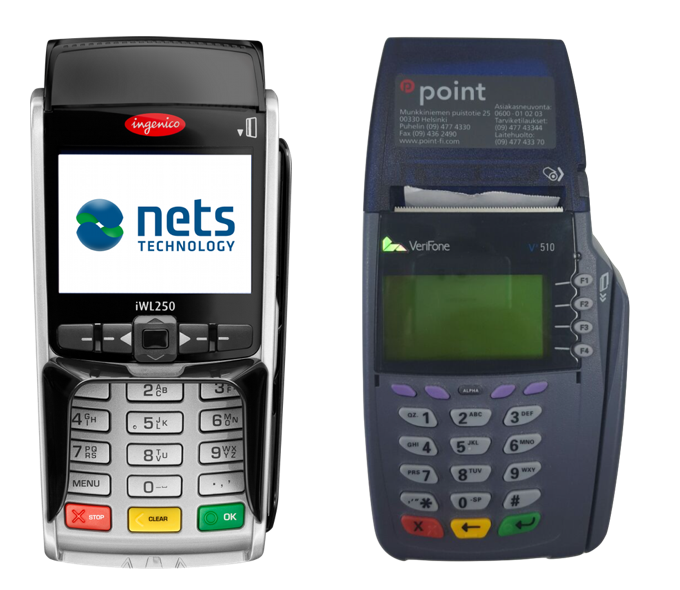
\includegraphics[width=8cm]{images/terminal1.png}
    \caption{Two examples of payment terminals from different manufacturers. Left image from: \url{http://www.netskauppa.fi/images/t/24-85-PrimaryImage.image.ashx}}
    \label{fig:terminals}
  \end{center}
\end{figure}

\begin{figure}[ht]
  \begin{center}
    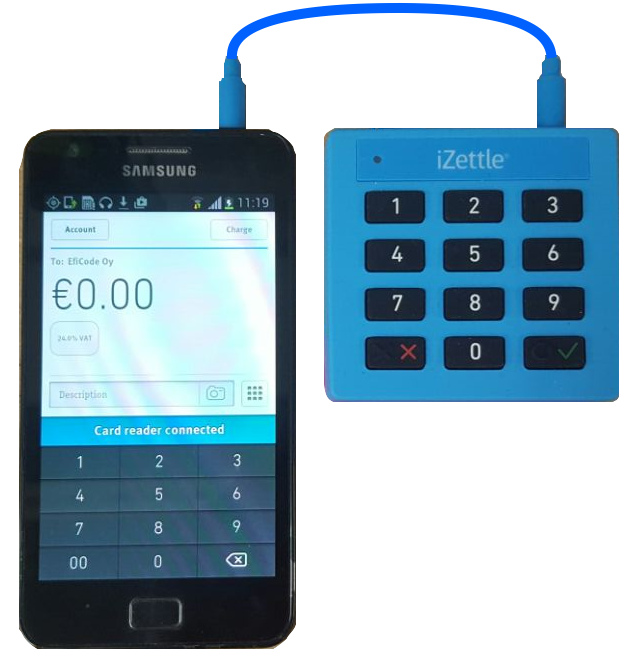
\includegraphics[width=7cm]{images/izettle.png}
    \caption{Example of a payment terminal which attaches to a smart phone.}
    \label{fig:izettle}
  \end{center}
\end{figure}

\section{Different approaches for test automation}

Problem of testing the payment terminal software in automated way can be viewed at different levels. Most abstract division can be seen if the testing is divided into two levels: white box testing and black box testing. White box testing is a method where source code is investigated and test cases are written to test the internal logic of the program. Black box testing on the other hand concentrates only on the inputs and the outputs of the software. Everything between those is not in a field of interest and black box testing only focuses on whether the right input produces the wanted output. (\emph{\cite{myers2011art}})

\emph{\cite{khan2012comparative}} distinguishes these methods clearly from each other by stating that white box testing is a process where full knowledge of source code is needed in order to write the tests. Black box testing is described in a way that only fundamental aspects of the application has to be known and black box testing has no or only little relevance to internal works of the program (\emph{\cite{pressman2005software}}). Black box testing techniques can be thus seen to apply for testing working product against the initial requirements of the software. In this way white box testing can be distinguished to cover unit and integration testing part of the software testing and the black box testing can be seen covering the acceptance testing part of the testing.

As black box testing is based only to the external exceptions and behavior of the software (\emph{\cite{khan2012comparative}}), acceptance testing of the payment terminal software can be seen to follow this methodology.

Therefore acceptance testing of a payment terminal software can be seen as a testing phase where the UI of the device and the use cases of the device are tested at the final production level, i.e. through using the real buttons of the device under test and observing that the expected messages can be seen through the screen of the device under test.

\section{Test suite syntax}

Test suite syntax plays significant role in automated acceptance testing environment of payment terminals in terms of test readability, reusability and adaptivity. When building automated acceptance testing environment, the tests should be understandable enough that whole development team and people related to the project can easily adopt the test syntax.

According to the well recognized guidelines of test automation by \emph{\cite{snakeoil}}, test automation and the process that it automates should be kept carefully separated. Test automation should be built in a form that it is easy to review and distinct from the process that it automates. These guidelines should be taken into account also when determining suitable test framework and test suite syntax.

When evaluating suitable test automation framework, it should be recognized, that shared knowledge is a key factor of successful test automation. Software projects usually involves some sort of quality assurance (QA) or even individual a QA team. Projects tend involve also fair amount of people with no technical background or coding skills and still their responsibilities involve guaranteeing the quality of the software. \emph{\cite{just_enough}} recognizes that high level test languages help to share the knowledge amongst the people that are responsible of the product. When information and knowledge is shared it helps in achieving the objectives of test automation and builds up the morale amongst the people that are involved.

\emph{\cite{lowell2003successful}} states that acceptance tests should be easy as possible to write or otherwise people working with the project will not write the tests as the task is seen unpleasant. Tests must be also easy to maintain and also people that have not written the tests should be able to modify the tests to suit updated program features. For this reason the test cases should be human readable and understandable also to non-technical people. Test steps should be self explanatory and unambiguous.

Test cases of a payment terminal software acceptance testing contain relatively high amount of repetition as for example test step of inserting PIN code is the same whether right or wrong PIN code is inserted or whether the test case would validate credit or debit payment. For this reason, test case syntax should be as modular as possible in order to allow reuse of keywords with different parameters. Easily reusable keywords also allows fast creation of new test cases.

Tests can be essentially written in some conventional coding language, for example Java or Python, or by using some higher level language. There are many widely used test frameworks available for conventional coding languages, for example jUnit for Java (\emph{\cite{junit}}). This, however, requires coding experience to some extend to be able to understand and write the tests or modify the existing ones. As it is stated above, combined with the guideline for writing tests understandable enough, usage of conventional coding languages can be seen opposing the best practices. On the other other hand, test case syntax must be versatile enough to accommodate different kinds of testing scenarios and needs. This leads to situation where the abstraction level of the test cases has to be considered thoroughly.

\begin{figure}[ht]
  \begin{center}
    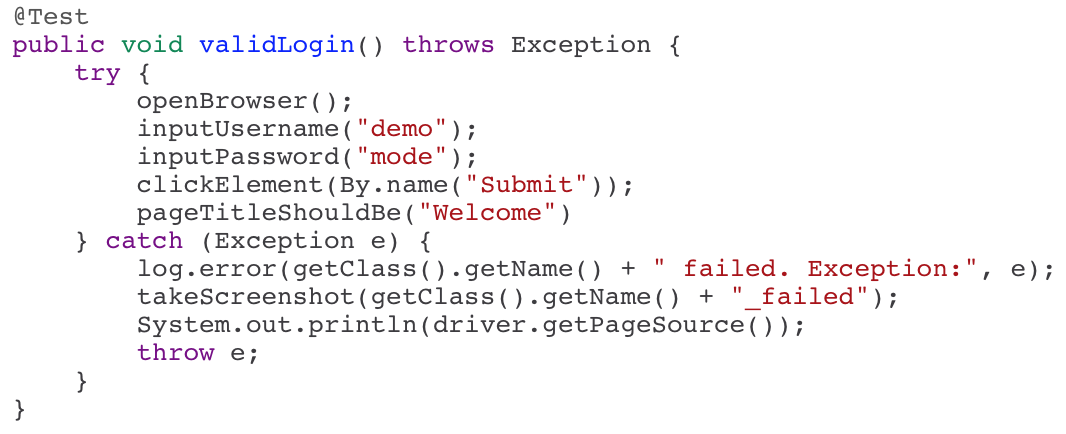
\includegraphics[width=13cm]{images/junit_example.png}
    \caption{Example of a jUnit test case that tries to login to website.}
    \label{fig:junit}
  \end{center}
\end{figure}
\FloatBarrier

In addition to the test frameworks utilizing the use of some conventional coding language for test cases, there are also couple of well recognized tests frameworks available that uses more human-like language for writing the tests. These frameworks usually use the same libraries for interacting with the system under test (SUT) as more low level frameworks but they allow more higher level syntax of the actual test scripts. One fairly popular example of this kind of more high level test framework is Cucumber. Cucumber is an open source acceptance test framework that utilizes behavior-driven development (BDD) style (\emph{\cite{cucumber}}). Cucumber uses Gherkin language that is designed to be human readable without previous knowledge of coding (\emph{\cite{gherkin}}). This means that also business oriented people involved with the project can understand the test cases.

\begin{figure}[ht]
  \begin{center}
    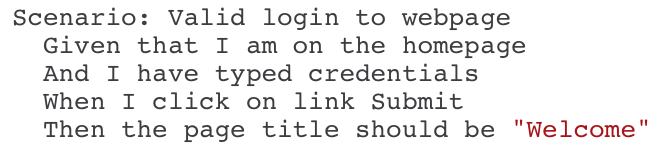
\includegraphics[width=8cm]{images/cucumber_example.png}
    \caption{Example of a simple Cucumber test scenario and use of Gherkin language.}
    \label{fig:cucumber}
  \end{center}
\end{figure}
\FloatBarrier

Another good example of higher level test frameworks is Robot Framework (RF). RF is an example of generic keyword driven test automation framework (\emph{\cite{robotframework}}). RF allows creation of human readable test cases and reusability and extendability of high-level keywords is made relatively easy (\emph{\cite{stresnjak2011usage}}). \emph{\cite{Rfuserguide}} also outlines that RF has highly modular software architecture allowing it to be easily connected to any kind of SUT by using different test libraries.

Example of a Robot Framework test case can be seen in Figure~\ref{fig:robot_example} bellow. It is easy to see the intended test case execution by looking the test case and this will be the goal for the environment proposed later on in this master's thesis.

\begin{figure}[ht]
  \begin{center}
    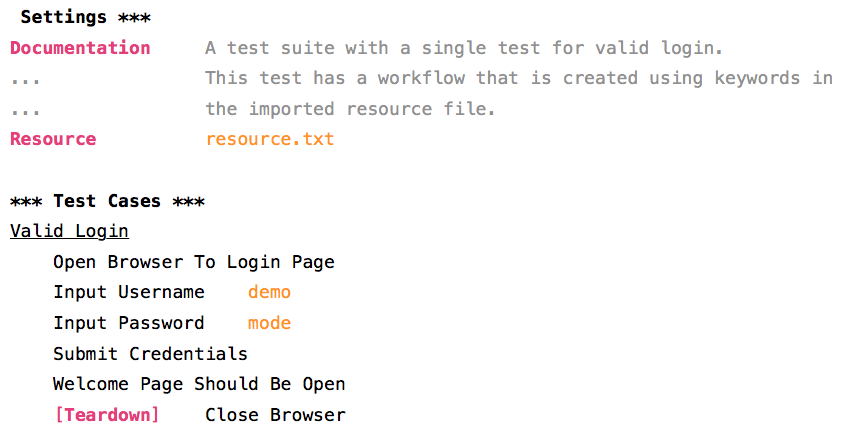
\includegraphics[width=12cm]{images/robot_example.png}
    \caption{Example of a simple test suite. Source: \url{http://robotframework.org}}
    \label{fig:robot_example}
  \end{center}
\end{figure}
\FloatBarrier
